\documentclass[answers]{exam}
\usepackage{marvosym}

%...TikZ & PGF
\usepackage{pgfplots}
\pgfplotsset{compat=1.11}
\tikzset{>=latex}
\usetikzlibrary{calc,math}
\usepackage{tikzsymbols}
\usepgfplotslibrary{fillbetween}
\usetikzlibrary{decorations.markings} 
\usetikzlibrary{arrows.meta} %...APP2 for arrows as objects and images
\usetikzlibrary{backgrounds} %...For shading portions of graphs
\usetikzlibrary{patterns} %...Unit 5 Problems
\usetikzlibrary{shapes.geometric} %...For drawing cylinders in Unit 2
\usepackage{makecell} %...use \thead{} to enable line skip in table headers
\tikzset{
    mark position/.style args={#1(#2)}{
        postaction={
            decorate,
            decoration={
                markings,
                mark=at position #1 with \coordinate (#2);
            }
        }
    }
} %...See https://tex.stackexchange.com/questions/43960/define-node-at-relative-coordinates-of-draw-plot

\tikzset{
    declare function = {trajectoryequation10(\x,\vi,\thetai)= tan(\thetai)*\x - 10*\x^2/(2*(\vi*cos(\thetai))^2);},
    declare function = {trajectoryequation(\x,\vi,\thetai)= tan(\thetai)*\x - 9.8*\x^2/(2*(\vi*cos(\thetai))^2);},
    declare function = {patheq(\x,\yi,\vi,\thetai)= \yi + tan(\thetai)*\x - 9.8*\x^2/(2*(\vi*cos(\thetai))^2);},
    declare function = {patheqten(\x,\yi,\vi,\thetai)= \yi + tan(\thetai)*\x - 10*\x^2/(2*(\vi*cos(\thetai))^2);} %like patheq but with gravity = 10
}

%...siunitx
\usepackage{siunitx}
\DeclareSIUnit{\nothing}{\relax}
\def\mymu{\SI{}{\micro\nothing} }
\DeclareSIUnit\mmHg{mmHg}
\DeclareSIUnit{\mile}{mi}
%...NOTE: "The product symbol between the number and unit is set using the quantity-product option."

%...Other
\usepackage{amsthm}
\usepackage{amsmath}
\usepackage{amssymb}
\usepackage{cancel}
\usepackage{subcaption}
\usepackage{dashrule}
\usepackage{enumitem}
\usepackage{fontawesome}
\usepackage{multicol}
\usepackage{glossaries}
%\numberwithin{equation}{section}
\numberwithin{figure}{section}
\usepackage{float}
\usepackage{twemojis} %...twitter emojis
\usepackage{utfsym}
\usepackage{linearb} %...For \BPwheel in Unit 8
\newcommand{\R}{\mathbb{R}} %...real number symbol
\usepackage{graphicx}
\graphicspath{ {../Figures/} }
\usepackage{hyperref}
\hypersetup{colorlinks=true,
    linkcolor=blue,
    filecolor=magenta,
    urlcolor=cyan,}
\urlstyle{same}
\newcommand{\hdashline}{{\hdashrule{\textwidth}{0.5pt}{0.8mm}}}
\newcommand{\hgraydashline}{{\color{lightgray} \hdashrule{0.99\textwidth}{1pt}{0.8mm}}}

%...Miscellaneous user-defined symbols
\newcommand{\fnet}{F_{\text{net}}} %...For net force
\newcommand{\bvec}[1]{\vec{\mathbf{#1}}} %...bold vector
\newcommand{\bhat}[1]{\,\hat{\mathbf{#1}}} %...bold hat vector
\newcommand{\que}{\mathord{?}}  %...Question mark symbol in equation env
%...Define thick horizontal rule for examples:
\newcommand{\hhrule}{\hrule\hrule}
\let\oldtexttt\texttt% Store \texttt
\renewcommand{\texttt}[2][black]{\textcolor{#1}{\ttfamily #2}}% 

%...For use in the exam document class
\newif\ifprintmetasolutions


%...Decreases space above and below align and gather enironment
\makeatletter
\g@addto@macro\normalsize{%
  \setlength\abovedisplayskip{-3pt}
  \setlength\belowdisplayskip{6pt} 
}
\makeatother





\usepackage[margin=1in]{geometry}
\usepackage[figurewithin=none]{caption}
\usepackage{exam-randomizechoices}
\setrandomizerseed{1}

\CorrectChoiceEmphasis{\color{red}\bfseries}
\renewcommand{\solutiontitle}{\noindent\textbf{\textcolor{red}{Solution:}}\enspace}

\usepackage{OutilsGeomTikz}
\usepackage{utfsym} %...Symbols in Unit 7 Problems
\usepackage{tabu} %...Symbols in Unit 7 Problems

%...For use in Unit 2            %    
\setlength{\columnsep}{2cm}      %
\setlength{\columnseprule}{1pt}  %
\usepackage[none]{hyphenat}      %
%%%%%%%%%%%%%%%%%%%%%%%%%%%%%%%%%

%...For use in Unit 11 on Waves:
\pgfdeclarehorizontalshading{visiblelight}{50bp}{  %
color(0.00000000000000bp)=(red);                   %
color(8.33333333333333bp)=(orange);                %
color(16.66666666666670bp)=(yellow);               %
color(25.00000000000000bp)=(green);                %
color(33.33333333333330bp)=(cyan);                 %
color(41.66666666666670bp)=(blue);                 %
color(50.00000000000000bp)=(violet)                %
}                                                  %

\newcommand{\checkbox}[1]{%
  \ifnum#1=1
    \makebox[0pt][l]{\raisebox{0.15ex}{\hspace{0.1em}\Large$\checkmark$}}%
  \fi
  $\square$%
}
%%%%%%%%%%%%%%%%%%%%%%%%%%%%%%%%%%%%%%%%%%%%%%%%%%%%

%...If using circuitikz package:
% \ctikzset{bipoles/battery1/height=0.5}
% \ctikzset{bipoles/battery1/width=0.25}
% \ctikzset{bipoles/resistor/height=0.15}
% \ctikzset{bipoles/resistor/width=0.4}
\usepackage{circuitikz}
\ctikzset{bipoles/battery1/height=0.5}
\ctikzset{bipoles/battery1/width=0.25}
\ctikzset{bipoles/battery/height=0.4}
\ctikzset{bipoles/battery/width=0.2}
\ctikzset{bipoles/resistor/height=0.17}
\ctikzset{bipoles/resistor/width=0.38}
\ctikzset{bipoles/capacitor/width=0.1}
\ctikzset{bipoles/capacitor/height=0.4}
\ctikzset{bipoles/cuteswitch/thickness=0.3,bipoles/cuteswitch/shape=circ}
\ctikzset{bipoles/bulb/height=0.4,bipoles/bulb/width=0.4}


\setrandomizerseed{1}
\bracketedpoints

\newif\ifversionKlevel

\versionKleveltrue

\header{Physics \\Test on Unit 9: Conservation of Charge}{}{Name:\enspace\makebox[5cm]{\hrulefill}}

\ifversionKlevel
    \header{Physics \\Test on Unit 9: Conservation of Charge}{}{Name:\enspace\makebox[5cm]{\hrulefill}}
\fi

\begin{document}

\begin{questions}

\question
All wires shown below are made of the same material. Which wires shown has the smallest resistance?

\begin{center}
\begin{tikzpicture}
\node[cylinder, 
	draw,
        % text={black!5},
	cylinder uses custom fill, 
	cylinder body fill = black!5, 
	cylinder end fill = black!20,
	minimum height = 2cm,
        minimum width=1cm] (c) at (0,0) {Wire 1};
    \node[xshift=-1pt] at (1,0) {$A$};
    \draw[|<->|,shift={(0,0.8)}] (-0.8,0) -- (1,0) node[above,pos=0.5] {$L$};
\end{tikzpicture}
\hspace{1cm}
\begin{tikzpicture}
\node[cylinder, 
	draw,
        % text={black!5},
	cylinder uses custom fill, 
	cylinder body fill = black!5, 
	cylinder end fill = black!20,
	minimum height = 2cm,
        minimum width=1.5cm] (c) at (0,0) {Wire 2};
    \draw[rounded corners=2mm] (0.9,0) -- (1.3,0.1) -- (1.6,0.25) node[right] {$2A$};
    \draw[|<->|,shift={(0,1)}] (-0.8,0) -- (1,0) node[above,pos=0.5] {$L$};
\end{tikzpicture}
\hspace{1cm}
\begin{tikzpicture}
\node[cylinder, 
	draw,
        % text={black!5},
	cylinder uses custom fill, 
	cylinder body fill = black!5, 
	cylinder end fill = black!20,
	minimum height = 4cm,
        minimum width=1cm] (c) at (0,0) {Wire 3};
    \node at (1.9,0) {$A$};
    \draw[|<->|,shift={(0,0.8)}] (-1.7,0) -- (1.9,0) node[above,pos=0.5] {$2L$};
\end{tikzpicture}
\end{center}

\medskip

\begin{randomizechoices}[norandomize]
    \choice Wire 1
    \correctchoice Wire 2
    \choice Wire 3
    \choice There is not enough information to tell. 
\end{randomizechoices}


\begin{solution}
Resistance is proportional to length and inversely proportional to surface area:

\begin{equation*}
    R \propto \frac{L}{A}
\end{equation*}

Therefore, the wire with the least length and greatest area will have the smallest resistance: Wire 2.
\end{solution}

\question
A positively charged rod touches a neutral metal sphere. The rod becomes less positive and the metal sphere now has an excess of positive charge. The redistribution of charge happens because \fillin[electrons] move from the sphere to the rod.

\begin{randomizechoices}
    \choice Neutrons
    \correctchoice Electrons
    \choice Atoms
    \choice Protons
\end{randomizechoices}

\question
Which of the charges shown in the image below is negative?

\begin{center}
    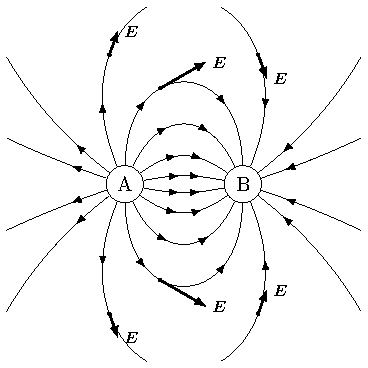
\includegraphics[width=6cm]{documents/figures/electric-field-lines-1.pdf}
\end{center}

\begin{randomizechoices}[norandomize]
    \choice A
    \correctchoice B
    \choice Both
    \choice Neither
\end{randomizechoices}

\question
According to Coulomb's Law, if you increase the charge on two objects the electrical force between them will

\begin{randomizechoices}[keeplast]
    \choice Stay the same
    \correctchoice Increase
    \choice Decrease
    \choice Not enough information 
\end{randomizechoices}

\question
What is the force between two charged spheres, each having a charge of $+\SI{2}{C}$, which are a distance of \SI{3}{m} apart?

\begin{randomizechoices}
    \choice \SI{9e9}{N}
    \choice \SI{4e9}{N}
    \correctchoice \SI{12e9}{N}
    \choice \SI{2e9}{N}
\end{randomizechoices}

\question
Two point charges, initially \SI{1}{cm} apart, are moved to a distance of \SI{3}{cm} apart. By what factor do the resulting electric and gravitational forces between them change?

\begin{randomizechoices}
    \choice The forces decrease by $1/3$.
    \correctchoice The forces decrease by $1/9$
    \choice The forces increase by $3$.
    \choice The forces increase by $9$
\end{randomizechoices}

\question
Electric fields point

\begin{randomizechoices}
    \correctchoice away from positive charge and towards negative charge
    \choice away from negative charge and towards positive charge
    \choice from left to right
    \choice away from the big charge and towards the little charge  
\end{randomizechoices}

\question
The diagram below shows two identical metal spheres, 1 and 2, separated by distance $d$. Each sphere has mass $m$ and possesses the charges shown below. The system consists of the two charges \underline{only}; the system does \textit{not} include the Earth.

\begin{center}
\begin{tikzpicture}
    \draw (0,0) circle (5mm) node {$+q$} node[below=5mm] {Sphere 1};
    \draw (5,0) circle (5mm) node {$+q$} node[below=5mm] {Sphere 2};
    \draw[|<->|,shift={(0,0.9)}] (0,0) -- (5,0) node[pos=0.5,above] {$d$};
\end{tikzpicture}
\end{center}

Which diagram best represents the electrostatic force $F_e$ and the gravitational force $F_g$ acting on Sphere~2 due to Sphere 1?

\begin{center}
\begin{tikzpicture}
    \fill (0,0) circle (5pt);
    \draw[yshift=+3pt,->] (0,0) -- (1,0) node[above] {$F_g$};
    \draw[yshift=-3pt,->] (0,0) -- (2,0) node[below] {$F_e$};
    \node[above=2pt] at (current bounding box.north) {Diagram A};
\end{tikzpicture}
\hspace{7mm}
\begin{tikzpicture}
    \draw[yshift=+3pt,->,white] (0,0) -- (1,0) node[above] {$F_g$}; %...FOR ALIGNMENT ONLY
    \draw[yshift=-3pt,->,white] (0,0) -- (1,0) node[below] {$F_e$}; %...FOR ALIGNMENT ONLY
    \fill (0,0) circle (5pt);
    \draw[->] (0,0) -- (1,0) node[above] {$F_g$};
    \draw[->] (0,0) -- (-2,0) node[below] {$F_e$};
    \node[above=2pt] at (current bounding box.north) {Diagram B};
\end{tikzpicture}
\hspace{7mm}
\begin{tikzpicture}
    \fill (0,0) circle (5pt);
    \draw[yshift=+3pt,->] (0,0) -- (-1,0) node[above] {$F_g$};
    \draw[yshift=-3pt,->] (0,0) -- (-2,0) node[below] {$F_e$};
    \node[above=2pt] at (current bounding box.north) {Diagram C};
\end{tikzpicture}
\hspace{7mm}
\begin{tikzpicture}
    \draw[yshift=+3pt,->,white] (0,0) -- (1,0) node[above] {$F_g$}; %...FOR ALIGNMENT ONLY
    \draw[yshift=-3pt,->,white] (0,0) -- (1,0) node[below] {$F_e$}; %...FOR ALIGNMENT ONLY
    \fill (0,0) circle (5pt);
    \draw[->] (0,0) -- (-1,0) node[above] {$F_g$};
    \draw[->] (0,0) -- (+2,0) node[below] {$F_e$};
    \node[above=2pt] at (current bounding box.north) {Diagram D};
\end{tikzpicture}
\end{center}

\begin{randomizeoneparchoices}[norandomize]
    \choice Diagram A
    \choice Diagram B
    \choice Diagram C
    \correctchoice Diagram D
\end{randomizeoneparchoices}

\question
The magnitude of the electrostatic force between two charged particles is directly proportional to the product of the magnitude of the charges and inversely proportional to the square of the distance between them. This statement best describes

\begin{randomizechoices}
    \correctchoice Coulomb's Law
    \choice Coulomb's Constant
    \choice Newton's 3rd Law
    \choice Newton's 2nd Law
    \choice Newton's 1st Law 
\end{randomizechoices}

\question
Which of the following labeled points is in the region with the greatest magnitude of electric field?

\begin{center}
    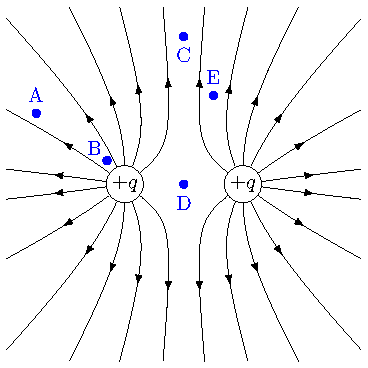
\includegraphics[width=6cm]{documents/figures/electric-field-lines-2.pdf}
\end{center}

\begin{randomizeoneparchoices}[norandomize]
    \choice Point A
    \correctchoice Point B
    \choice Point C
    \choice Point D
    \choice Point E
\end{randomizeoneparchoices}

\question
Which diagram shows a series circuit?

\begin{center}
\begin{minipage}{4.4cm}
\centering
\begin{tikzpicture}[x=1.5cm,y=1.8cm]
    \draw (0,0) to[battery1] (0,1) -- (1,1) to[R={$R_1$}] (1,0);
    \draw (1,1) -- (2,1) to[R={$R_2$}] (2,0) -- (0,0); 
    \node[above=4pt] at (current bounding box.north) {Circuit A};
\end{tikzpicture}
\end{minipage}%
\begin{minipage}{3.4cm}
\centering
\begin{tikzpicture}[x=1.2cm,y=1.8cm]
    \draw (0,0) to[battery1] (2,0) to[R={$R_2$}] (2,1) -- (0,1) to[R={$R_1$}] (0,0);
    \node[above=4pt] at (current bounding box.north) {Circuit B};
\end{tikzpicture}
\end{minipage}%
\begin{minipage}{3.5cm}
\centering
\begin{tikzpicture}[x=1.8cm,y=1.8cm]
    \draw (0,0) to[battery1] (0,1) -- (1,1) -- (1,0) -- (0,0);
    \begin{scope}[shift={(0.7,0.25)},x=1cm,y=1cm]
        \small
        \ctikzset{bipoles/resistor/height=0.12}
        \ctikzset{bipoles/resistor/width=0.3}
        \fill[white] (0,0) rectangle (1,1);
        \draw (0,0) to[R={$R_1$}] (0,1) -- (1,1) to[R={$R_2$}] (1,0) -- (0,0);
    \end{scope}
    \node[above=4pt,xshift=-2em] at (current bounding box.north) {Circuit C};
\end{tikzpicture}
\end{minipage}%
\begin{minipage}{3cm}
\centering
\begin{tikzpicture}[x=1cm,y=1.8cm]
    \draw (0,0) to[R,l_={$R_2$}] (2,0) -- (2,1) to[R,l_={$R_1$}] (0,1) -- (0,0);
    \draw (2,0.5) to[battery1] (0,0.5);
    \node[above=4pt] at (current bounding box.north) {Circuit D};
\end{tikzpicture}
\end{minipage}
\end{center}

\scalebox{0}{
\begin{randomizeoneparchoices}[norandomize]
    \choice Circuit A
    \correctchoice Circuit B
    \choice Circuit C
    \choice Circuit D
\end{randomizeoneparchoices}
}

\question
A circuit is set up as show below.  What is wrong with the figure?

\begin{center}
\begin{tikzpicture}[x=3cm,y=1.5cm]
    \draw (0,0) to[battery1] (0,1) -- (1,1) -- (1,0);
    \draw (0,0) to[cute open switch] (1,0);
    \begin{scope}[shift={(0.5,1.1)}]
        \foreach \x in {20,40,...,160}{
            \draw[thick,rotate=\x] (0,0) -- (0.3,0);
        }
        \fill[white] (0,0.11) circle (3.5mm);
        \node at (0,0) {\resizebox{5mm}{!}{\faLightbulbO}};
    \end{scope}
\end{tikzpicture}
\end{center}

\begin{randomizechoices}[keeplast]
    \correctchoice The switch is open but the light bulb is on.
    \choice  The light bulb will short the circuit.
    \choice No power supply is shown.
    \choice Nothing is wrong with the image.
\end{randomizechoices}

\question
A light bulb has a resistance of \SI{1.2}{\ohm}. What is the voltage across the light bulb when a current of \SI{4}{A} flows through it?

\begin{randomizeoneparchoices}
    \correctchoice \SI{4.8}{V}
    \choice \SI{0.3}{V}
    \choice \SI{3.3}{V}
    \choice \SI{5.2}{V}
\end{randomizeoneparchoices}

\clearpage

\question
Initially, a \SI{75}{W} light bulb operates at a voltage of \SI{120}{V}. If the bulb wattage was doubled, what would happen to current through the battery?

\begin{randomizechoices}[keeplast]
    \correctchoice The current would double.
    \choice The current would stay the same.
    \choice The current would be halved.
    \choice There is not enough information to tell.
\end{randomizechoices}

\begin{solution}
The power dissipated by a circuit element is

\begin{equation*}
    P=IV
\end{equation*}

Therefore, doubling the power while keeping voltage constant requires that the current through the element be doubled too.
\end{solution}

\question
What kind of circuit is shown below?

\begin{center}
\begin{tikzpicture}[x=1.8cm,y=1.5cm]
    \draw (0,1) to[battery,l_={\SI{8}{V}}] (0,0) -- (1,0) to[R,l_={\SI{4}{\ohm}}] (1,1) to[R,l_={\SI{5}{\ohm}}] (0,1);
    \draw (1,0) -- (2,0) to[R,l_={\SI{4}{\ohm}}] (2,1) -- (1,1);
\end{tikzpicture}
\end{center}

\begin{randomizeoneparchoices}
    \choice Short circuit
    \choice Series circuit
    \correctchoice Combination circuit
    \choice Parallel circuit
\end{randomizeoneparchoices}

\question
Your house is wired in

\begin{randomizechoices}
    \choice parallel, so that if something is unplugged everything else goes off.
    \choice series, so that if something is unplugged everything else goes off.
    \correctchoice parallel, so that if something is unplugged everything else is fine.
    \choice series, so that is something is unplugged everything else is fine.
\end{randomizechoices}

\question
A 125 volt battery delivers a current of 2.0 amperes to a portable radio. If the resistance in the circuit was doubled, what would happen to the current?

\begin{randomizechoices}[keeplast]
    \choice The current would remain the same.
    \correctchoice There current would be cut in half.
    \choice The current would double.
    \choice There is not enough information to tell.
\end{randomizechoices}

\begin{solution}
Ohm's law states

\begin{equation*}
    I = \frac{V}{R}
\end{equation*}

Therefore, if resistance is doubled while voltage remains constant, the current must decrease by one-half.
\end{solution}

\question
Three resistors, \SI{4}{\ohm}, \SI{6}{\ohm}, and \SI{8}{\ohm}, are connected in parallel in an electric circuit. The equivalent resistance $R_\mathrm{eq}$ of the circuit is
\bigskip

\begin{randomizeoneparchoices}
    \choice $\SI{4}{\ohm} < R_\mathrm{eq} < \SI{8}{\ohm}$
    \choice $R_\mathrm{eq} = \SI{18}{\ohm}$
    \correctchoice $R_\mathrm{eq} < \SI{4}{\ohm}$
    \choice $\SI{10}{\ohm} < R_\mathrm{eq} < \SI{19}{\ohm}$
\end{randomizeoneparchoices}

% \begin{randomizechoices}
%     \choice Between \SI{4}{\ohm} and \SI{8}{\ohm} 
%     \choice \SI{18}{\ohm}
%     \choice Between \SI{10}{\ohm} and \SI{19}{\ohm}
%     \correctchoice Less than \SI{4}{\ohm}
% \end{randomizechoices}

\question
Which combination of resistors has the smallest equivalent resistance?

\begin{center}
\begin{minipage}{3.8cm}
\centering
\begin{tikzpicture}[x=1.5cm]
    \draw (0,0) to[R,l_={\SI{1}{\ohm}}] (1,0) to[R,l_={\SI{1}{\ohm}}] (2,0);
    \fill (0,0) circle (2pt);
    \fill (2,0) circle (2pt);
    \phantom{%...for alignment only
        \begin{scope}[shift={(0.5,-0.5)}]
            \fill[white] (0,0) rectangle (1,1);
            \draw (0,0) -- (0,1) to[R={\SI{0}{\ohm}}] (1,1) -- (1,0) to[R={\SI{0}{\ohm}}]  (0,0);
        \end{scope}
    }
    \node[above=2pt] at (current bounding box.north) {Circuit A};
\end{tikzpicture}
\end{minipage}%
\begin{minipage}{3.8cm}
\centering
\begin{tikzpicture}[x=1.5cm]
    \draw (0,0) -- (2,0);
    \begin{scope}[shift={(0.5,-0.5)}]
        \fill[white] (0,0) rectangle (1,1);
        \draw (0,0) -- (0,1) to[R={\SI{2}{\ohm}}] (1,1) -- (1,0) to[R={\SI{2}{\ohm}}]  (0,0);
    \end{scope}
    \fill (0,0) circle (2pt);
    \fill (2,0) circle (2pt);
    \node[above=2pt] at (current bounding box.north) {Circuit B};
\end{tikzpicture}
\end{minipage}
\begin{minipage}{3.8cm}
\centering
\begin{tikzpicture}[x=1.5cm]
    \draw (0,0) -- (2,0);
    \begin{scope}[shift={(0.5,-0.5)}]
        \fill[white] (0,0) rectangle (1,1);
        \draw (0,0) -- (0,1) to[R={\SI{1}{\ohm}}] (1,1) -- (1,0) to[R={\SI{1}{\ohm}}]  (0,0);
    \end{scope}
    \fill (0,0) circle (2pt);
    \fill (2,0) circle (2pt);
    \node[above=2pt] at (current bounding box.north) {Circuit C};
\end{tikzpicture}
\end{minipage}
\begin{minipage}{3.8cm}
\centering
\begin{tikzpicture}[x=1.5cm]
    \draw (0,0) to[R,l_={\SI{2}{\ohm}}] (1,0) to[R,l_={\SI{2}{\ohm}}] (2,0);
    \fill (0,0) circle (2pt);
    \fill (2,0) circle (2pt);
    \phantom{%...for alignment only
        \begin{scope}[shift={(0.5,-0.5)}]
            \fill[white] (0,0) rectangle (1,1);
            \draw (0,0) -- (0,1) to[R={\SI{0}{\ohm}}] (1,1) -- (1,0) to[R={\SI{0}{\ohm}}]  (0,0);
        \end{scope}
    }
    \node[above=2pt] at (current bounding box.north) {Circuit D};
\end{tikzpicture}
\end{minipage}
\end{center}

\scalebox{0}{
\begin{randomizeoneparchoices}[norandomize]
    \choice Circuit A
    \choice Circuit B
    \correctchoice Circuit C
    \choice Circuit D
\end{randomizeoneparchoices}
}

\begin{solution}
The equivalent resistance in the parallel Circuit C is

\begin{equation*}
    R_\mathrm{eq} = \left(\frac{1}{\SI{1}{\ohm}} + \frac{1}{\SI{1}{\ohm}}\right)^{-1} = \SI{0.5}{\ohm}
\end{equation*}

All other circuits have bigger equivalent resistances.
\end{solution}

\question
In the diagram below, if the circuit breaks at Point 1, which light bulb(s) remain on?

\begin{center}
\begin{tikzpicture}[y=1.8cm]
    \draw (0,0) to[battery] (0,1) -- (3,1) -- (3,0) -- (0,0);
    \draw (1,1) -- (1,0);
    \draw (2,1) -- (2,0);
    \draw (1,0.4) node[fill=white] {\faLightbulbO} node[above left=2pt] {X};
    \draw (2,0.4) node[fill=white] {\faLightbulbO} node[above left=2pt] {Y};
    \draw (3,0.4) node[fill=white] {\faLightbulbO} node[above left=2pt] {Z};
    \fill (2,0.8) circle (2pt);
    \draw[<-,thick,shift={(2pt,2pt)}] (2,0.8) -- ++(0.6,0.4) node[right] {Point 1};
\end{tikzpicture}
\end{center}

\begin{randomizeoneparchoices}
    \choice X and Y
    \correctchoice X and Z
    \choice Y and Z
    \choice None of them
\end{randomizeoneparchoices}









\end{questions}


\end{document}